\documentclass[table]{beamer}
\usepackage{beamerthemesplit}
\usetheme{boxes}
\usecolortheme{seahorse}
% \useinnertheme{myboxes}
% \usepackage{amsmath}
% \usepackage[fleqn]{amsmath}
\usepackage{ifthen}
\usepackage{xspace}
\usepackage{multirow}
\usepackage{booktabs}
\usepackage{xcolor}
\usepackage[style=nature]{biblatex}
\bibliography{../manuscripts/bib/references}
\newrobustcmd*{\footlessfullcite}{\AtNextCite{\renewbibmacro{title}{}\renewbibmacro{in:}{}}\footfullcite}
\AtEveryBibitem{\clearfield{month}}
\AtEveryCitekey{\clearfield{month}}

% Make all footnotes smaller
\renewcommand{\footnotesize}{\scriptsize}

\definecolor{myGray}{gray}{0.9}
\colorlet{rowred}{red!30!white}

\setbeamertemplate{blocks}[rounded][shadow=true]

\setbeamercolor{defaultcolor}{bg=structure!30!normal text.bg,fg=black}
\setbeamercolor{block body}{bg=structure!30!normal text.bg,fg=black}
\setbeamercolor{block title}{bg=structure!50!normal text.bg,fg=black}

\newenvironment<>{varblock}[2][\textwidth]{%
  \setlength{\textwidth}{#1}
  \begin{actionenv}#3%
    \def\insertblocktitle{#2}%
    \par%
    \usebeamertemplate{block begin}}
  {\par%
    \usebeamertemplate{block end}%
  \end{actionenv}}

\newenvironment{displaybox}[1][\textwidth]
{
    \centerline\bgroup\hfill
    \begin{beamerboxesrounded}[lower=defaultcolor,shadow=true,width=#1]{}
}
{
    \end{beamerboxesrounded}\hfill\egroup
}

\newenvironment{onlinebox}[1][4cm]
{
    \newbox\mybox
    \newdimen\myboxht
    \setbox\mybox\hbox\bgroup%
        \begin{beamerboxesrounded}[lower=defaultcolor,shadow=true,width=#1]{}
    \centering
}
{
    \end{beamerboxesrounded}\egroup
    \myboxht\ht\mybox
    \raisebox{-0.25\myboxht}{\usebox\mybox}\hspace{2pt}
}

\newenvironment{mydescription}{
    \begin{description}
        \setlength{\leftskip}{-1.5cm}}
    {\end{description}}

\newenvironment{myitemize}{
    \begin{itemize}
        \setlength{\leftskip}{-.3cm}}
    {\end{itemize}}

% define formatting for footer
\newcommand{\myfootline}{%
    {\it
    \insertshorttitle
    \hspace*{\fill} 
    \insertshortauthor, \insertshortinstitute
    % \ifx\insertsubtitle\@empty\else, \insertshortsubtitle\fi
    \hspace*{\fill}
    \insertframenumber/\inserttotalframenumber}}

% set up footer
\setbeamertemplate{footline}{%
    \usebeamerfont{structure}
    \begin{beamercolorbox}[wd=\paperwidth,ht=2.25ex,dp=1ex]{frametitle}%
        \Tiny\hspace*{4mm}\myfootline\hspace{4mm}
    \end{beamercolorbox}}

% remove navigation bar
\beamertemplatenavigationsymbolsempty


% \newcommand{\change}[1]{{\color{blue} #1}\xspace}
\newcommand{\change}[1]{{\color{black} #1}\xspace}


\newcommand{\citationNeeded}{\textcolor{magenta}{\textbf{[CITATION NEEDED!]}}\xspace}
\newcommand{\tableNeeded}{\textcolor{magenta}{\textbf{[TABLE NEEDED!]}}\xspace}
\newcommand{\figureNeeded}{\textcolor{magenta}{\textbf{[FIGURE NEEDED!]}}\xspace}
\newcommand{\highLight}[1]{\textcolor{magenta}{\MakeUppercase{#1}}}

\newcommand{\editorialNote}[1]{\textcolor{red}{[\textit{#1}]}}
\newcommand{\ignore}[1]{}
\newcommand{\addTail}[1]{\textit{#1}.---}
\newcommand{\super}[1]{\ensuremath{^{\textrm{#1}}}}
\newcommand{\sub}[1]{\ensuremath{_{\textrm{#1}}}}
\newcommand{\dC}{\ensuremath{^\circ{\textrm{C}}}}

\providecommand{\e}[1]{\ensuremath{\times 10^{#1}}}

\newcommand{\mthnote}[2]{{\color{red} #2}}

\newcommand{\ifTwoArgs}[3]{\ifthenelse{\equal{#1}{}\or\equal{#2}{}}{}{#3}\xspace}
\newcommand{\ifArg}[2]{\ifthenelse{\equal{#1}{}}{}{#2}\xspace}

\newcommand{\allDatasets}{\ensuremath{\mathcal{\alignment{}{}}}\xspace}
\newcommand{\allParameterValues}{\ensuremath{\boldsymbol{\Theta}}\xspace}
\newcommand{\bayesfactor}[2]{\ensuremath{BF_{#1\protect\ifArg{#2}{,}#2}}}
\newcommand{\given}{\ensuremath{\,|\,}\xspace}
\newcommand{\msb}{\upshape\texttt{\MakeLowercase{ms\MakeUppercase{B}ayes}}\xspace}
\newcommand{\hky}{HKY85\xspace}
\newcommand{\uniformMin}[1]{\ensuremath{a_{#1}}\xspace}
\newcommand{\uniformMax}[1]{\ensuremath{b_{#1}}\xspace}
\newcommand{\locusRateHetShapeParameter}{\ensuremath{\alpha}\xspace}
\newcommand{\ancestralThetaVector}{\ensuremath{\boldsymbol{\theta_{A}}}\xspace}
\newcommand{\descendantThetaVector}[1]{\ensuremath{\boldsymbol{\theta_{D#1}}}\xspace}
\newcommand{\divtscaledvector}{\ensuremath{\mathbf{{\divtscaled{}{}}}}\xspace}
\newcommand{\divtvector}{\ensuremath{\boldsymbol{\divt{}}}\xspace}
\newcommand{\divtuniquevector}{\ensuremath{\mathbf{\divtunique{}}}\xspace}
\newcommand{\bottleTimeVector}{\ensuremath{\boldsymbol{\bottleTime{}}}\xspace}
\newcommand{\bottleTime}[1]{\ensuremath{\divt{B\ifArg{#1}{,}#1}}\xspace}
\newcommand{\bottleScalarVector}[1]{\ensuremath{\boldsymbol{\bottleScalar{#1}{}}}\xspace}
\newcommand{\bottleScalar}[2]{\ensuremath{\zeta_{D#1\protect\ifArg{#2}{,}#2}}\xspace}
\newcommand{\migrationRateVector}{\ensuremath{\mathbf{\migrationRate{}}}\xspace}
\newcommand{\geneTreeVector}{\ensuremath{\mathbf{\geneTree{}{}}}\xspace}
\newcommand{\alignmentVector}{\ensuremath{\mathbf{\alignment{}{}}}\xspace}
\newcommand{\alignment}[2]{\ensuremath{X_{#1\protect\ifTwoArgs{#1}{#2}{,}#2}}\xspace}
\newcommand{\geneTree}[2]{\ensuremath{G_{#1\protect\ifTwoArgs{#1}{#2}{,}#2}}\xspace}
\newcommand{\migrationRate}[1]{\ensuremath{m_{#1}}\xspace}
\newcommand{\recombinationRate}{\ensuremath{r}\xspace}
\newcommand{\ploidyScalar}[2]{\ensuremath{\rho_{#1\protect\ifTwoArgs{#1}{#2}{,}#2}}\xspace}
\newcommand{\ploidyScalarVector}{\ensuremath{\boldsymbol{\ploidyScalar{}{}}}\xspace}
\newcommand{\descendantRelativeThetaVector}[1]{\ensuremath{\boldsymbol{\eta_{D#1}}}\xspace}
\newcommand{\descendantRelativeTheta}[2]{\ensuremath{\eta_{D#1\protect\ifArg{#2}{,}#2}}\xspace}
\newcommand{\mutationRateScalarConstant}[2]{\ensuremath{\nu_{#1\protect\ifTwoArgs{#1}{#2}{,}#2}}\xspace}
\newcommand{\mutationRateScalarConstantVector}{\ensuremath{\boldsymbol{\mutationRateScalarConstant{}{}}}\xspace}
\newcommand{\locusMutationRateScalar}[1]{\ensuremath{\upsilon_{#1}}\xspace}
\newcommand{\locusMutationRateScalarVector}{\ensuremath{\boldsymbol{\upsilon}}\xspace}
\newcommand{\hkyModel}[2]{\ensuremath{\phi_{#1\protect\ifTwoArgs{#1}{#2}{,}#2}}\xspace}
\newcommand{\hkyModelVector}{\ensuremath{\boldsymbol{\hkyModel{}{}}}\xspace}
\newcommand{\mutationRate}{\ensuremath{\mu}\xspace}
\newcommand{\iid}{\textit{iid}\xspace}
\newcommand{\model}[1]{\ensuremath{\Theta}\xspace}
\newcommand{\npairs}[1]{\ensuremath{Y_{#1}}}
\newcommand{\nloci}[1]{\ensuremath{k_{#1}}\xspace}
\newcommand{\nlociTotal}{\ensuremath{K}\xspace}
\newcommand{\myTheta}[1]{\ensuremath{\theta_{#1}}}
\newcommand{\ancestralTheta}[1]{\ensuremath{\theta_{A\protect\ifArg{#1}{,}#1}}\xspace}
\newcommand{\descendantTheta}[2]{\ensuremath{\theta_{D#1\protect\ifArg{#2}{,}#2}}\xspace}
\newcommand{\meanDescendantTheta}[1]{\ensuremath{\descendantTheta{}{#1}}\xspace}
\newcommand{\nucdiv}[1]{\ensuremath{\pi_{#1}}}

\newcommand{\ssVector}[1]{\ensuremath{\mathbf{\alignmentSS{#1}{}}}\xspace}
\newcommand{\ssVectorObs}{\ensuremath{\ssVector{}^*}\xspace}
\newcommand{\ssSpace}{\ensuremath{\euclideanSpace{\ssVectorObs}}\xspace}
\newcommand{\ssVectorObsPLS}{\ensuremath{\ssVectorObs_{PLS}}\xspace}
\newcommand{\alignmentSS}[2]{\ensuremath{S_{#1\protect\ifTwoArgs{#1}{#2}{,}#2}}\xspace}
\newcommand{\alignmentSSObs}[2]{\ensuremath{\alignmentSS{#1}{#2}^*}\xspace}
\newcommand{\tol}{\ensuremath{\epsilon}\xspace}
\newcommand{\euclideanSpace}[1]{\ensuremath{B_{\tol}(#1)}\xspace}
\newcommand{\hpvector}[1]{\ensuremath{\Lambda_{#1}}}
\newcommand{\divtscaled}[2]{\ensuremath{t_{#1\protect\ifTwoArgs{#1}{#2}{,}#2}}}
\newcommand{\divt}[1]{\ensuremath{\tau_{#1}}}
\newcommand{\divtunique}[1]{\ensuremath{T_{#1}}}
\newcommand{\ssMatrix}{\ensuremath{\mathbb \alignmentSS{}{}}\xspace}
\newcommand{\ssMatrixRaw}[1]{\ensuremath{{\ssMatrix}_{stats#1}}\xspace}
\newcommand{\ssMatrixPLS}[1]{\ensuremath{{\ssMatrix}_{PLS#1}}\xspace}
\newcommand{\hpmatrix}[1]{\ensuremath{\mathcal{P}_{#1}}}
\newcommand{\meant}[2]{\ensuremath{E(\divt{#1})_{#2}}}
\newcommand{\meantestimate}{\ensuremath{\hat{E(\divt{})}}\xspace}
\newcommand{\vart}[2]{\ensuremath{Var(\divt{#1}{})_{#2}}}
\newcommand{\vmratio}[1]{\ensuremath{\Omega_{#1}}}
\newcommand{\numt}[1]{\ensuremath{\Psi_{#1}}}
\newcommand{\probnumt}[2]{\ensuremath{p(\numt{#1} = {#2})}}
\newcommand{\postprobnumt}[1]{\ensuremath{p(\numt{} = {#1}|\ssSpace)}}
\newcommand{\postprobnumtnot}[1]{\ensuremath{p(\numt{} \neq {#1}|\ssSpace)}}
\newcommand{\postprobomegasimult}{\ensuremath{p(\vmratio{} < 0.01 | \ssSpace)}\xspace}
\newcommand{\modelprior}[1]{\ensuremath{f(\model{})}}
\newcommand{\modelpost}[1]{\ensuremath{f(\model{}|\ssSpace)}}
\newcommand{\npriorsamples}{\ensuremath{n}\xspace}
\newcommand{\globalcoalunit}{\ensuremath{4\globalpopsize}\xspace}
\newcommand{\globalpopsize}{\ensuremath{N_C}\xspace}
\newcommand{\effectivePopSize}[1]{\ensuremath{N_e{#1}}\xspace}
\newcommand{\coalunit}{\ensuremath{4\effectivePopSize{}}\xspace}
\newcommand{\priorsample}[1]{\ensuremath{\hpmatrix{\modelprior{}}}}
\newcommand{\truncprior}[1]{\ensuremath{\hpmatrix{\tol}}\xspace}
\newcommand{\postsample}[1]{\ensuremath{\hpmatrix{\modelpost{}}}}
\newcommand{\abcllr}[1]{ABC\sub{LLR}}
\newcommand{\abcglm}[1]{ABC\sub{GLM}}
\newcommand{\integerPartition}[1]{\ensuremath{a({#1})}}
\newcommand{\uniqueModel}[2]{\ensuremath{M_{#1\protect\ifTwoArgs{#1}{#2}{,}#2}}}
\newcommand{\taxonLocusVector}[1]{\ensuremath{\{#1{1}{1},\ldots,#1{\npairs{}}{\nloci{\npairs{}}}\}}\xspace}
\newcommand{\taxonVector}[1]{\ensuremath{\{#1{1},\ldots,#1{\npairs{}}\}}\xspace}
\newcommand{\locusVector}[1]{\ensuremath{\{#1{1},\ldots,#1{\nlociTotal}\}}\xspace}

\newcommand{\simulationDescription}[2]{\change{Each plot represents #1
    simulation replicates using the same $#2$ samples from the prior}}
\newcommand{\simulationDistribution}{\ensuremath{\divt{} \sim U(0,
    \divt{max})}\xspace}
\newcommand{\estimateDescription}[2]{All estimates were obtained using #1 and #2}
\newcommand{\estimateDescriptionUncorrected}[1]{All estimates based on
    unadjusted posterior, \truncprior{}, obtained using #1}
\newcommand{\priorDescription}[4]{Prior settings were \priorSettings{#1}{#2}{#3}{#4}}
\newcommand{\priorSettings}[4]{$\divt{} \sim U(0, #1)$,
    $\meanDescendantTheta{} \sim U(#2, #3)$, and
    $\ancestralTheta{}{} \sim U(#2, #4)$}
\newcommand{\priorDescriptionBug}[4]{Prior settings were
    \priorSettingsBug{#1}{#2}{#3}{#4}}
\newcommand{\priorSettingsBug}[4]{$\divt{} \sim U(0, #1)$,
    $\meanDescendantTheta{} \sim U(#2, #3)$, and
    $\ancestralTheta{}{} \sim U(0.01, #4)$}
\newcommand{\simulationScheme}{simulations where \divt{} (in \globalcoalunit
    generations) for 22 population pairs is drawn from a series of uniform
    distributions, \simulationDistribution}
\newcommand{\captionPowerOmega}{Histograms of the estimated dispersion index
    of divergence times ($\hat{\vmratio{}}$) from \simulationScheme.
    The threshold for one divergence event \citep{Hickerson2006} is indicated
    by the dashed line, and the estimated probability of inferring one
    divergence event, $p(\hat{\vmratio{}}\le 0.01)$, is given for each
    \divt{max}}
\newcommand{\captionPowerPsiMode}{Histograms of the estimated number of
    divergence events ($\hat{\numt{}}$) from \simulationScheme.
    The estimated probability of inferring one divergence event,
    $p(\hat{\numt{}} = 1)$, is given for each \divt{max}}
\newcommand{\captionPowerPsi}{Histograms of the estimated posterior
    probability of one divergence event, \postprobnumt{1}, from
    \simulationScheme.
    The estimated probability of inferring one divergence event with a
    Bayes factor greater than 10 (dashed black line),
    $p(\bayesfactor{\numt{}=1}{\numt{} \ne 1} > 10)$, is given for each \divt{max}.
    The red line indicates $\postprobnumt{1} = 0.95$, and the estimated
    probability of inferring a posterior probability greater than 0.95 is given
    to the right of the line.}
\newcommand{\captionAccuracy}[1]{Accuracy and precision of #1 estimates from
    \simulationScheme.
    The proportion of estimates less than the true value ($p(\hat{#1}<#1)$) is
    given for each \divt{max}}
\newcommand{\samplingErrorTableNote}{An estimate of 1.0 for a posterior probability
    is an artifact of sampling error}


\newcommand{\refAccuracyALL}[1]{\labelcref{fig_acc_t_ss_llr_bug,fig_acc_t_ss_glm_bug,fig_acc_t_pls_llr_bug,fig_acc_t_pls_glm_bug,fig_acc_o_ss_llr_bug,fig_acc_o_ss_glm_bug,fig_acc_o_pls_llr_bug,fig_acc_o_pls_glm_bug}}
\newcommand{\refAccuracySS}[1]{\labelcref{fig_acc_t_ss_llr_bug,fig_acc_t_ss_glm_bug,fig_acc_o_ss_llr_bug,fig_acc_o_ss_glm_bug}}
\newcommand{\refAccuracySSfull}[1]{\labelcref{fig_acc_t_ssfull_llr_bug,fig_acc_t_ssfull_glm_bug,fig_acc_o_ssfull_llr_bug,fig_acc_o_ssfull_glm_bug}}
\newcommand{\refSSfull}[1]{\labelcref{fig_acc_t_ssfull_llr_bug,fig_acc_t_ssfull_glm_bug,fig_acc_o_ssfull_llr_bug,fig_acc_o_ssfull_glm_bug,fig_pow_o_ssfull_llr_bug,fig_pow_o_ssfull_glm_bug,fig_pow_psi_modes_ssfull_glm_bug}}
\newcommand{\refSS}[1]{\labelcref{fig_acc_t_ss_llr_bug,fig_acc_t_ss_glm_bug,fig_acc_o_ss_llr_bug,fig_acc_o_ss_glm_bug,fig_pow_o_ss_llr_bug,fig_pow_o_ss_glm_bug,fig_pow_psi_ss}}
\newcommand{\refAccuracyPLS}[1]{\labelcref{fig_acc_t_pls_llr_bug,fig_acc_t_pls_glm_bug,fig_acc_o_pls_llr_bug,fig_acc_o_pls_glm_bug}}
\newcommand{\refAccuracySScorrected}[1]{\labelcref{fig_acc_t_ss_llr_bug,fig_acc_t_ss_glm_bug,fig_acc_o_ss_llr_bug,fig_acc_o_ss_glm_bug}}
\newcommand{\refAccuracyPLScorrected}[1]{\labelcref{fig_acc_t_pls_llr_bug,fig_acc_t_pls_glm_bug,fig_acc_o_pls_llr_bug,fig_acc_o_pls_glm_bug}}
\newcommand{\refAccuracyUncorrected}[1]{\labelcref{fig_acc_t_ss_unc,fig_acc_t_pls_unc,fig_acc_o_ss_unc,fig_acc_o_pls_unc}}
\newcommand{\refAccuracyCorrected}[1]{\labelcref{fig_acc_t_ss_llr_bug,fig_acc_t_ss_glm_bug,fig_acc_t_pls_llr_bug,fig_acc_t_pls_glm_bug,fig_acc_o_ss_llr_bug,fig_acc_o_ss_glm_bug,fig_acc_o_pls_llr_bug,fig_acc_o_pls_glm_bug}}
\newcommand{\refAccuracyGLM}[1]{\labelcref{fig_acc_t_ss_glm_bug,fig_acc_t_pls_glm_bug,fig_acc_o_ss_glm_bug,fig_acc_o_pls_glm_bug}}
\newcommand{\refAccuracyLLR}[1]{\labelcref{fig_acc_t_ss_llr_bug,fig_acc_t_pls_llr_bug,fig_acc_o_ss_llr_bug,fig_acc_o_pls_llr_bug}}
\newcommand{\refAccuracyOmega}[1]{\labelcref{fig_acc_o_ss_llr_bug,fig_acc_o_ss_glm_bug,fig_acc_o_pls_llr_bug,fig_acc_o_pls_glm_bug}}
\newcommand{\refAccuracyOmegaUncorrected}[1]{\labelcref{fig_acc_o_ss_unc,fig_acc_o_pls_unc}}
\newcommand{\refAccuracyOmegaCorrected}[1]{\labelcref{fig_acc_o_ss_llr_bug,fig_acc_o_ss_glm_bug,fig_acc_o_pls_llr_bug,fig_acc_o_pls_glm_bug}}
\newcommand{\refAccuracyTime}[1]{\labelcref{fig_acc_t_ss_llr_bug,fig_acc_t_ss_glm_bug,fig_acc_t_pls_llr_bug,fig_acc_t_pls_glm_bug}}

\newcommand{\tn}{\tabularnewline}

\newcommand{\widthFigure}[5]{\begin{figure}[htbp]
\begin{center}
    \includegraphics[width=#1\textwidth]{#2}
    \captionsetup{#3}
    \caption{#4}
    \label{#5}
    \end{center}
    \end{figure}}

\newcommand{\heightFigure}[5]{\begin{figure}[htbp]
\begin{center}
    \includegraphics[height=#1]{#2}
    \captionsetup{#3}
    \caption{#4}
    \label{#5}
    \end{center}
    \end{figure}}

\newcommand{\mFigure}[3]{\widthFigure{1.0}{#1}{listformat=figList}{#2}{#3}\clearpage}
\newcommand{\siFigure}[3]{\widthFigure{1.0}{#1}{name=Figure S, labelformat=noSpace, listformat=sFigList}{#2}{#3}\clearpage}



% \title[Caution for ABC model choice]{Evidence for climate-driven
%     diversification?}
% \subtitle{A caution for interpreting ABC inferences of simultaneous historical
%     events}
% \title[ABC model choice]{ABC, not as easy as 1,2,3}
\title[Islands and Integrals]{Islands and Integrals}
% \subtitle{The potential perils of model choice via approximate Bayesian
%     computation}
\subtitle{Processes of Diversification in an Island Archipelago and Bayesian
    Methods of Comparative Phylogeographical Model Choice}

\author[J.\ Oaks]{
    Jamie R.\ Oaks\inst{1} %\and
    % Jeet Sukumaran\inst{2} \and
    % Jacob A.\ Esselstyn\inst{3} \and
    % Charles W.\ Linkem\inst{4} \and
    % Cameron D.\ Siler\inst{5} \and
    % Mark T.\ Holder\inst{1} \and
    % Rafe M.\ Brown\inst{1}
}
\institute[University of Kansas]{
    \inst{1}%
        University of Kansas
    % \and
    % \inst{2}%
    %     Duke University
    % \and
    % \inst{3}%
    %     Louisiana State University
    % \and
    % \inst{4}%
    %     University of Washington
    % \and
    % \inst{5}%
    %     University of Oklahoma
}

% \date{\today}
\date{October 16, 2013}

\begin{document}
\maketitle

\begin{frame}
\frametitle{Outline}
\tableofcontents
\end{frame}

% \section{Intro}
% \begin{frame}
% \frametitle{Table of Contents}
% \tableofcontents[currentsection]
% \end{frame}

% \section{An empirical application of ABC model choice}
\section{Southeast Asia---A biogeographer's paradise}

{
\usebackgroundtemplate{\includegraphics[width=\paperwidth]{images/maps/se-asia-present.png}}
\begin{frame}
    \frametitle{Southeast Asia}    
\end{frame}
}

{
\usebackgroundtemplate{\includegraphics[width=\paperwidth]{images/maps/se-asia-120.png}}
\begin{frame}
    \frametitle{Southeast Asia}    
\end{frame}
}

\subsection{Philippines---Pleistocene model of diversification}

\begin{frame}
    \frametitle{Philippine Archipelago}
    \begin{center}
        \includegraphics<1>[width=.5\textwidth]{images/maps/Philippines-present.png}
        \includegraphics<2>[width=.5\textwidth]{images/maps/Philippines.png}
    \end{center}
\end{frame}

\begin{frame}
    \frametitle{PAIC model}
    \begin{columns}[c]
        \column{.5\textwidth}
            \begin{myitemize}
                \item Repeated coalescence and fragmentation of Pleistocene
                    Aggregate Island Complexes (PAICs)
                \item Prominent paradigm for explaining Philippine biodiversity
                \item Proposed as model of diversification
                \begin{myitemize}
                    \item Limited testing
                \end{myitemize}
            \end{myitemize}
        \column{.5\textwidth}
            \includegraphics[width=\textwidth]{images/maps/Philippines.png}
    \end{columns}
\end{frame}

\section{Testing the Pleistocene model of diversification}

\begin{frame}
    \frametitle{PAIC model: Previous work}
    \begin{columns}[c]
        \column{.5\textwidth}
            \begin{myitemize}
            \item Phylogenetic work
                \begin{myitemize}
                \item Are groups of species reciprocally monophyletic among
                    PAICs?
                \item Do most divergences date to the Pleistocene?
                \end{myitemize}
            \item Population genetic work
                \begin{myitemize}
                \item Are islands within PAICs responsible for most of the
                    genetic diversity?
                \end{myitemize}
            \end{myitemize}

            All of these approaches are really asking if PAIC cycles were
            responsible for a large proportion of diversity in the Philippines.
        \column{.5\textwidth}
            \includegraphics[width=\textwidth]{images/maps/Philippines.png}
    \end{columns}
\end{frame}

\begin{frame}
    \frametitle{PAIC model: A new approach}
    % \begin{columns}[c]
    %     \column{.5\textwidth}
            \begin{mydescription}
                \item[$H_0$] Repeated island fragmentation promoted diversification
                    among island populations
                    \begin{mydescription}
                        \item[Prediction] Temporal distribution of divergences
                            between inter-island populations within PAICs
                            should be temporally clustered and correspond with
                            interglacial rises in sea level
                    \end{mydescription}
                \item[$H_1$] Island fragmentation did not promote diversification
                    \begin{mydescription}
                        \item[Prediction] Inter-island diversification was
                            dispersal mediated; no temporal clustering
                    \end{mydescription}
            \end{mydescription}
            
            {\bf Key pattern:} The temporal distribution of divergences
                    among species distributed across PAIC islands
        % \column{.5\textwidth}
        %     \includegraphics[width=\textwidth]{images/maps/Philippines.png}
    % \end{columns}
\end{frame}

\subsection{The data}

\begin{frame}
\frametitle{Outline}
\tableofcontents[currentsection,currentsubsection]
\end{frame}

\begin{frame}
\begin{columns}[c]
    \column{.5\textwidth}
        \begin{table}%[htbp]
            \scriptsize
            \addtolength{\tabcolsep}{-0.09cm}
            \def\firstrowcolor{}
            \def\secondrowcolor{}
            \def\thirdrowcolor{}
            \def\fourthrowcolor{}
            \def\fifthrowcolor{}
            \only<2>{\def\firstrowcolor{\rowcolor{rowred}}}
            \only<3>{\def\secondrowcolor{\rowcolor{rowred}}}
            \only<4>{\def\thirdrowcolor{\rowcolor{rowred}}}
            \only<5>{\def\fourthrowcolor{\rowcolor{rowred}}}
            \only<6>{\def\fifthrowcolor{\rowcolor{rowred}}}
            \centering
            \begin{tabular}{ l c c }
                % \toprule
                \textbf{Species} & {\boldmath $n_1$} & {\boldmath $n_2$} \\
                \hline
                \textbf{\textsc{Mammals}} & & \\
                \fifthrowcolor  \emph{Crocidura beatus}             & 12 & 11 \\
                \firstrowcolor  \emph{Crocidura negrina-panayensis} & 12 & 6  \\
                \thirdrowcolor  \emph{Hipposideros obscurus}        & 19 & 9  \\
                \secondrowcolor \emph{Hipposideros pygmaeus}        & 3  & 12 \\
                \thirdrowcolor  \emph{Cynopterus brachyotis}        & 20 & 8  \\
                \firstrowcolor  \emph{Cynopterus brachyotis}        & 8  & 14 \\
                \thirdrowcolor  \emph{Haplonycteris fischeri}       & 29 & 8  \\
                \firstrowcolor  \emph{Haplonycteris fischeri}       & 9  & 21 \\
                \thirdrowcolor  \emph{Macroglossus minimus}         & 19 & 4  \\
                \firstrowcolor  \emph{Macroglossus minimus}         & 8  & 10 \\
                \thirdrowcolor  \emph{Ptenochirus jagori}           & 4  & 7  \\
                \firstrowcolor  \emph{Ptenochirus jagori}           & 8  & 8  \\
                \thirdrowcolor  \emph{Ptenochirus minor}            & 30 & 9  \\
                \textbf{\textsc{Squamates}} & & \\
                \fifthrowcolor  \emph{Cyrtodactylus gubaot-sumuroi} & 29 & 6  \\
                \secondrowcolor \emph{Cyrtodactylus annulatus}      & 14 & 3  \\
                \firstrowcolor  \emph{Cyrtodactylus philippinicus}  & 6  & 14 \\
                \firstrowcolor  \emph{Gekko mindorensis}            & 8  & 11 \\
                \firstrowcolor  \emph{Insulasaurus arborens}        & 22 & 10 \\
                \fourthrowcolor \emph{Pinoyscincus jagori}          & 8  & 8  \\
                \firstrowcolor  \emph{Dendrelaphis marenae}         & 6  & 6  \\
                \textbf{\textsc{Anurans}}  & & \\
                \secondrowcolor \emph{Limnonectes leytensis}        & 4  & 2  \\
                \secondrowcolor \emph{Limnonectes magnus}           & 2  & 3  \\
                \hline
            \end{tabular}
        \end{table}
    \column{.5\textwidth}
        \includegraphics<1>[width=\textwidth]{images/maps/Philippines.png}
        \includegraphics<2>[width=\textwidth]{images/maps/Philippines-negros_panay.png}
        \includegraphics<3>[width=\textwidth]{images/maps/Philippines-bohol_mindanao.png}
        \includegraphics<4>[width=\textwidth]{images/maps/Philippines-leyte_mindanao.png}
        \includegraphics<5>[width=\textwidth]{images/maps/Philippines-mindanao_samar.png}
        \includegraphics<6>[width=\textwidth]{images/maps/Philippines-leyte_samar.png}
\end{columns}
\end{frame}

\subsection{The method---approximate Bayesian model choice}

\begin{frame}
\frametitle{Outline}
\tableofcontents[currentsection,currentsubsection]
\end{frame}

\begin{frame}
    \frametitle{The method: \msb}
        Now we have genetic data for $\npairs{}=22$ taxon pairs, and we need to
        infer the distribution of their relative divergence times (\divt{})
        \[
            \divtvector = \{\divt{1},\divt{2},\ldots,\divt{\npairs{}}\}
        \]
        where \numt{} is the number of \emph{unique} divergence times
        within \divtvector
        % \begin{center}
        %     {\bf -OR-}
        % \end{center}
        % \[
        %     \divtuniquevector = \{\divtunique{1},\divtunique{2},\ldots,\divtunique{\npairs{}}\}
        % \]
        % where $\divtunique{i} \in \{ 1,2,\ldots,\numt{} \}$ and
        % $\mathbf{t}  = \{t_1, t_2,\ldots,t_{\numt{}}\}$ \\

        \begin{myitemize}
            \item We want to infer \numt{} and \divtvector from our data.
            \item This is a problem of model choice.
            \begin{myitemize}
                \item Bayesian framework is an attractive approach
                \item \msb uses an approximate Bayesian approach to estimate the
                    posterior probability of competing divergence models
            \end{myitemize}
        \end{myitemize}
\end{frame}

\begin{frame}
    \frametitle{Bayesian framework}
    Given sequence alignments \alignmentVector and: \\
        \begin{mydescription}
            \item[\divtvector] The vector of divergence times for each pair of populations
            \item[\numt{}] The number of unique divergence times within \divtvector
            \item[\model{}] The demographic and mutational parameters
        \end{mydescription}
    % \smallskip
    \begin{displaybox}[7.5cm]
    \[
        f(\numt{}, \divtvector, \model{} \given \alignmentVector) = 
        \frac{f(\alignmentVector \given \numt{}, \divtvector, \model{})
        f(\numt{}, \divtvector, \model{})}
        {f(\alignmentVector)}
    \]\vspace{0mm}
    \end{displaybox}
    \smallskip
    \[ \alignmentVector \to \ssVectorObs \]
    % \smallskip
    \begin{displaybox}[9.5cm]
    \[
        f(\numt{}, \divtvector, \model{} \given \euclideanSpace{\ssVectorObs}) = 
        \frac{f(\euclideanSpace{\ssVectorObs} \given \numt{}, \divtvector, \model{})
        f(\numt{}, \divtvector, \model{})}
        {f(\euclideanSpace{\ssVectorObs})}
    \]\vspace{0mm}
    \end{displaybox}

\end{frame}

\begin{frame}[b]
    \frametitle{The \msb model}
    \only<3>{
        \begin{mydescription}
            \item[\divtvector] The vector of divergence times for each pair of populations
            \item[\numt{}] The number of unique divergence times within \divtvector
            \item[\vmratio{}] The variance of \divtvector
        \end{mydescription}
        \vspace{1cm}
            % \divtvector The vector of divergence times for each pair of populations \\
            % \numt{} The number of unique divergence times withing \divtvector
    }
    \begin{onlyenv}<1-2>
    \begin{block}{\it Full Model:}
    {\tiny
    \begin{equation*}
        \begin{split}
        & f(\geneTreeVector,
        \numt{},
        \divtvector, \ancestralThetaVector,
        \descendantThetaVector{1}, \descendantThetaVector{2},
        \locusRateHetShapeParameter,
        \locusMutationRateScalarVector,
        \bottleTimeVector, \bottleScalarVector{1},
        \bottleScalarVector{2},
        \migrationRateVector \given
        \alignmentVector, \hkyModelVector, \ploidyScalarVector,
        \mutationRateScalarConstantVector) \\
        & = \frac{1}{f(\alignmentVector)}
        f(\numt{}) f(\divtvector \given \numt{})
        f(\locusRateHetShapeParameter)
        \Bigg[
        \prod_{i=1}^{\npairs{}}
        f(\ancestralTheta{i})
        f(\descendantTheta{1}{i}, \descendantTheta{2}{i})
        f(\bottleTime{i})
        f(\bottleScalar{1}{i}) f(\bottleScalar{2}{i})
        f(\migrationRate{i}) \\
        &
        \prod_{j=1}^{\nloci{i}}
        f(\alignment{i}{j} \given
        \geneTree{i}{j}, \hkyModel{i}{j})
        f(\geneTree{i}{j} \given
        \divt{i},
        \ancestralTheta{i}, \descendantTheta{1}{i}, \descendantTheta{2}{i},
        \ploidyScalar{i}{j}, \mutationRateScalarConstant{i}{j},
        \locusMutationRateScalar{j},
        \bottleTime{i}, \bottleScalar{1}{i}, \bottleScalar{2}{i},
        \migrationRate{i})
        \Bigg]
        \Bigg[
        \prod_{j=1}^{\nlociTotal}
        f(\locusMutationRateScalar{j} \given \locusRateHetShapeParameter)
        \Bigg]
        \label{eq:fullmodel}
        \end{split}
    \end{equation*}
    }
    \end{block}
    \end{onlyenv}
    % \pause
    % \vspace{1mm}
    \begin{block}<2->{\it Approximate Model:}
    {\tiny
    \begin{equation*}
        \begin{split}
        & f(\geneTreeVector,
        \numt{},
        \divtvector, \ancestralThetaVector,
        \descendantThetaVector{1}, \descendantThetaVector{2},
        \locusRateHetShapeParameter,
        \locusMutationRateScalarVector,
        \bottleTimeVector, \bottleScalarVector{1},
        \bottleScalarVector{2},
        \migrationRateVector \given
        \euclideanSpace{\ssVectorObs}, \hkyModelVector, \ploidyScalarVector,
        \mutationRateScalarConstantVector) \\
        & = \frac{1}{f(\euclideanSpace{\ssVectorObs})}
        f(\numt{}) f(\divtvector{} \given \numt{})
        f(\locusRateHetShapeParameter)
        \Bigg[
        \prod_{i=1}^{\npairs{}}
        f(\ancestralTheta{i})
        f(\descendantTheta{1}{i}, \descendantTheta{2}{i})
        f(\bottleTime{i})
        f(\bottleScalar{1}{i}) f(\bottleScalar{2}{i})
        f(\migrationRate{i}) \\
        &
        \prod_{j=1}^{\nloci{i}}
        f(\euclideanSpace{\alignmentSSObs{i}{j}} \given
        \geneTree{i}{j}, \hkyModel{i}{j})
        f(\geneTree{i}{j} \given
        \divt{i},
        \ancestralTheta{i}, \descendantTheta{1}{i}, \descendantTheta{2}{i},
        \ploidyScalar{i}{j}, \mutationRateScalarConstant{i}{j},
        \locusMutationRateScalar{j},
        \bottleTime{i}, \bottleScalar{1}{i}, \bottleScalar{2}{i},
        \migrationRate{i})
        \Bigg]
        \Bigg[
        \prod_{j=1}^{\nlociTotal}
        f(\locusMutationRateScalar{j} \given \locusRateHetShapeParameter)
        \Bigg]
        \label{eq:approxmodel}
        \end{split}
    \end{equation*}
    }
    \end{block}
\end{frame}

\section{Empirical results}
\subsection{To good to be true?}

\begin{frame}
\frametitle{Outline}
\tableofcontents[currentsection,currentsubsection]
\end{frame}

\begin{frame}
    \frametitle{Empirical results}
    \begin{columns}[c]
        \column{.4\textwidth}
            {\small
            Strong support for simultaneous divergence of all 22 taxon pairs \\
            \vspace{1cm}
            pp $>$ 0.96 \\
            \vspace{1cm}
            $\sim$100,000--250,000 years ago}
        \column{.6\textwidth}
        \includegraphics[width=\textwidth]{images/jointDensityPlots.jpg}
    \end{columns}
\end{frame}

\section{Simulation-based assessment of method}

\begin{frame}
\frametitle{Outline}
\tableofcontents[currentsection,currentsubsection]
\end{frame}

\begin{frame}
    \frametitle{Simulation-based power analyses}
    What is ``simultaneous''?
    \begin{myitemize}
        \item Draw divergence times from $U(0, \divt{max})$
        \item \divt{max} was set to:
            0.1, 0.2, 0.3, 0.4, 0.5, 0.6, 0.7, 0.8, 0.9, 1.0, 1.1, 1.2, 1.3,
            1.4, 1.5, 2.0, and 3.0
        \item Units are \globalcoalunit generations
    \end{myitemize}
\end{frame}

\begin{frame}
    \frametitle{Simulation results: Accuracy}
    \centerline{
    \includegraphics[height=8cm]{images/SS_accuracy_omega_modes_GLM.pdf}}
\end{frame}

\begin{frame}
    \frametitle{Simulation results: Power}
    \centerline{
    \includegraphics[height=8cm]{images/SS_power_psi_modes_GLM.pdf}}
\end{frame}

\begin{frame}
    \frametitle{Simulation results: Summary}
    Estimates of highly clustered divergences when divergence times are random
    over the past 7.5 million generations \\
    \bigskip
    More than 5\% of replicates estimate strong support (BF $>$ 10) for
    extreme case of one divergence when divergences are random over past 3
    million generations \\
    \bigskip
    More than 5\% of replicates estimate extreme case of one divergence based
    on \vmratio{} when divergences are random over past 2 million generations
\end{frame}

\subsection{Why the odd behavior?}

\begin{frame}
\frametitle{Outline}
\tableofcontents[currentsection,currentsubsection]
\end{frame}

\begin{frame}
    \frametitle{Causes of bias}
    Potential causes of the bias:
    \begin{enumerate}
        \item Uniform priors on parameters and model marginal likelihoods
        \item The prior on divergence models
        \item Theoretical limits of ABC model choice
    \end{enumerate}
\end{frame}

\begin{frame}
    \frametitle{Causes of bias: Marginal likelihoods}
    Models with more divergence events have lower marginal likelihoods \\
    \bigskip
    \begin{displaybox}[5.5cm]
        \small
        \[
            p(X) = \int_{\theta} p(X
            \given \theta) p(\theta) \mathrm{d}\theta
        \]%\vspace{0mm}
    \end{displaybox}
    \bigskip
    Broad uniform priors on nuisance parameters can hinder marginal likelihoods
    of rich models \\
\end{frame}

\begin{frame}
    \frametitle{Causes of bias: Marginal likelihoods}
    \begin{displaybox}[5.5cm]
        \small
        \[
            p(X) = \int_{\theta} p(X
            \given \theta) p(\theta) \mathrm{d}\theta
        \]%\vspace{0mm}
    \end{displaybox}
    \smallskip
    \centerline{
        \includegraphics<1>[height=6.5cm]{images/marginal-plot-2d-no-priors.pdf}
        \includegraphics<2>[height=6.5cm]{images/marginal-plot-2d-uniform-prior.pdf}
        \includegraphics<3>[height=6.5cm]{images/marginal-plot-2d.pdf}}
\end{frame}

\begin{frame}
    \frametitle{Causes of bias: Marginal likelihoods}
    % \begin{displaybox}[5.5cm]
    %     \small
    %     \[
    %         p(X) = \int_{\theta} p(X
    %         \given \theta) p(\theta) \mathrm{d}\theta
    %     \]%\vspace{0mm}
    % \end{displaybox}
    % \smallskip
    \centerline{
        \includegraphics<1>[height=8.0cm]{images/marginal-plot-3d-bare.pdf}
        \includegraphics<2>[height=8.0cm]{images/marginal-plot-3d-prior.pdf}
        \includegraphics<3>[height=8.0cm]{images/marginal-plot-3d.pdf}}
\end{frame}

\begin{frame}
    \frametitle{Causes of bias: Marginal likelihoods}
    Testing prior sensitivity \\
    \begin{enumerate}
        \item Assess behavior when priors are correct
        \item Assess behavior under ideal real-world priors
    \end{enumerate}
\end{frame}

\begin{frame}
    \frametitle{Causes of bias: Marginal likelihoods}
    \centerline{
    \includegraphics[height=8cm]{images/posterior_vs_true_prob.pdf}}
\end{frame}

\begin{frame}
    \frametitle{Causes of bias: Marginal likelihoods}
    \begin{center}
        \includegraphics[height=6cm]{images/SS_accuracy_omega_modes_GLM_inform10.pdf} \quad
        \includegraphics[height=6cm]{images/SS_power_psi_modes_GLM_inform10.pdf}
    \end{center}
\end{frame}

\begin{frame}
    \frametitle{Causes of bias: Marginal likelihoods}
    Marginal likelihoods are at least partially responsible for bias\\
    \bigskip
    However, when uniform priors are narrower than possible in a real-world
    setting, the bias remains
    \bigskip
    \begin{block}<2>{\it Potential solution:}
        Use more flexible parametric distributions on nuisance parameters (e.g., gamma)
    \end{block}
\end{frame}

\begin{frame}
    \frametitle{Causes of bias: Marginal likelihoods}
    \begin{block}{\it Potential solution:}
        Use more flexible parametric distributions on nuisance parameters (e.g., gamma)
    \end{block}
    \smallskip
    \centerline{
    \includegraphics[height=5.5cm]{images/likelihood-vs-prior-vs-belief-example.pdf}}
\end{frame}

\begin{frame}
    \frametitle{Causes of bias: Hyper-prior on models}
    \msb uses discrete uniform prior on the number of divergence events
    (\numt{})\\
    \bigskip
    This creates prior on divergence models that disfavors models with
    intermediate number of events\\
    \bigskip
    \centerline{
    \includegraphics[width=\textwidth]{images/partition_numbers.pdf}}
\end{frame}

\begin{frame}
    \frametitle{Causes of bias: Theoretical limits of ABC}
    When summary statistics are insufficient for discriminating among models,
    ABC is inconsistent estimator of model posterior probabilities
    \footlessfullcite{Robert2011}\\
    \bigskip
    True even if statistics are sufficient for each model\\
\end{frame}

\section{Conclusions}

\begin{frame}
\frametitle{Outline}
\tableofcontents[currentsection,currentsubsection]
\end{frame}

\begin{frame}
    \frametitle{Conclusions}
    Empirical results strongly support PAIC model \\
    \bigskip
    Based on simulations this is likely spurious \\
    \bigskip
    Low power and bias preclude any biological interpretation \\
    \bigskip
    Bias likely caused by combination of uniform priors on nuisance parameters
    and prior on model classes \\
    \bigskip
    \begin{block}{\it Potential Solutions:}
        \begin{enumerate}
            \item Flexible parametric distributions on nuisance parameters (e.g., gamma)
            \item More uniform prior over models (e.g., Dirichlet process)
        \end{enumerate}
    \end{block}
\end{frame}

\begin{frame}
    \frametitle{Recommendations}
    For Bayesian model choice, choose prior distributions carefully\\
    \bigskip
    All ABC model choice estimates should be accompanied by:
    \begin{enumerate}
        \item Simulation-based power analyses
        \item Assessment of prior sensitivity
    \end{enumerate}
    \medskip
\end{frame}

\section{An improved approach to the problem}

\begin{frame}
    \frametitle{PAIC model: Still needs testing}
    \begin{columns}[c]
        \column{.5\textwidth}
            What now? \\
            \begin{enumerate}
                \item Methodological advancements
                \begin{enumerate}
                    \item Extend \msb
                    \item Develop new fully Bayesian method
                \end{enumerate}
                \item Collect more data
            \end{enumerate}
        \column{.5\textwidth}
            \includegraphics[width=\textwidth]{images/maps/Philippines.png}
    \end{columns}
\end{frame}

\subsection{Improving existing and developing new method}

\begin{frame}
    \frametitle{Extend \msb}
    \begin{myitemize}
        \item Implement flexible prior options for demographic parameters
        \item Implement a better prior over divergence models
        \begin{enumerate}
            \item Uniform prior over divergence models (rather than \numt{})
            \item Dirichlet process prior
        \end{enumerate}
    \end{myitemize}
\end{frame}

\begin{frame}
    \frametitle{Novel Bayesian method}
    \includegraphics<1>[width=\textwidth]{images/model-cartoon-masked.pdf}
    \includegraphics<2>[width=\textwidth]{images/model-cartoon.pdf}
\end{frame}

\subsection{More data---a lot more}

\begin{frame}
    \frametitle{Genomic data}
    \begin{columns}[c]
        \column{.5\textwidth}
        \begin{myitemize}
            \item Collecting genomic data from two gekkonid radiations
                co-distributed throughout most of Philippine Archipelago
            \begin{myitemize}
                \item \emph{Cyrtodactylus}---12 species
                \item \emph{Gekko}---13 species
            \end{myitemize}
            \item Whole genome assemblies for each genus
            \item RAD-seq libraries constructed for $\sim130$ individuals
                from each genus
        \end{myitemize}
        \column{.5\textwidth}
        \includegraphics[width=\textwidth]{images/cyrt-agusanensis.jpg} \quad
        \includegraphics[width=\textwidth]{images/gekko-mindorensis.jpg}
    \end{columns}
\end{frame}


\begin{frame}
    \frametitle{Acknowledgments}
    \begin{columns}[c]
        \column{.5\textwidth}
            {\bf Ideas and feedback:}
            \begin{myitemize}
                \item KU Herpetology
                \item Holder Lab
                \item Melissa Callahan
                \item Mike Hickerson
                \item Laura Kubatko
            \end{myitemize}
        \column{.5\textwidth}
            {\bf Funding:}
            \begin{myitemize}
                \item NSF
                \item KU EEB \& BI
            \end{myitemize}
            {\bf Computation:}
            \begin{myitemize}
                \item KU ITTC
                \item KU Computing Center
            \end{myitemize}
    \end{columns}
\end{frame}

% Extra slides

\begin{frame}[noframenumbering]
    \frametitle{Geological history}
    \includegraphics[width=\textwidth]{images/maps/arees-fig3.png}
\end{frame}
    
\begin{frame}[noframenumbering]
    \frametitle{Gene tree divergences}
    \centerline{
    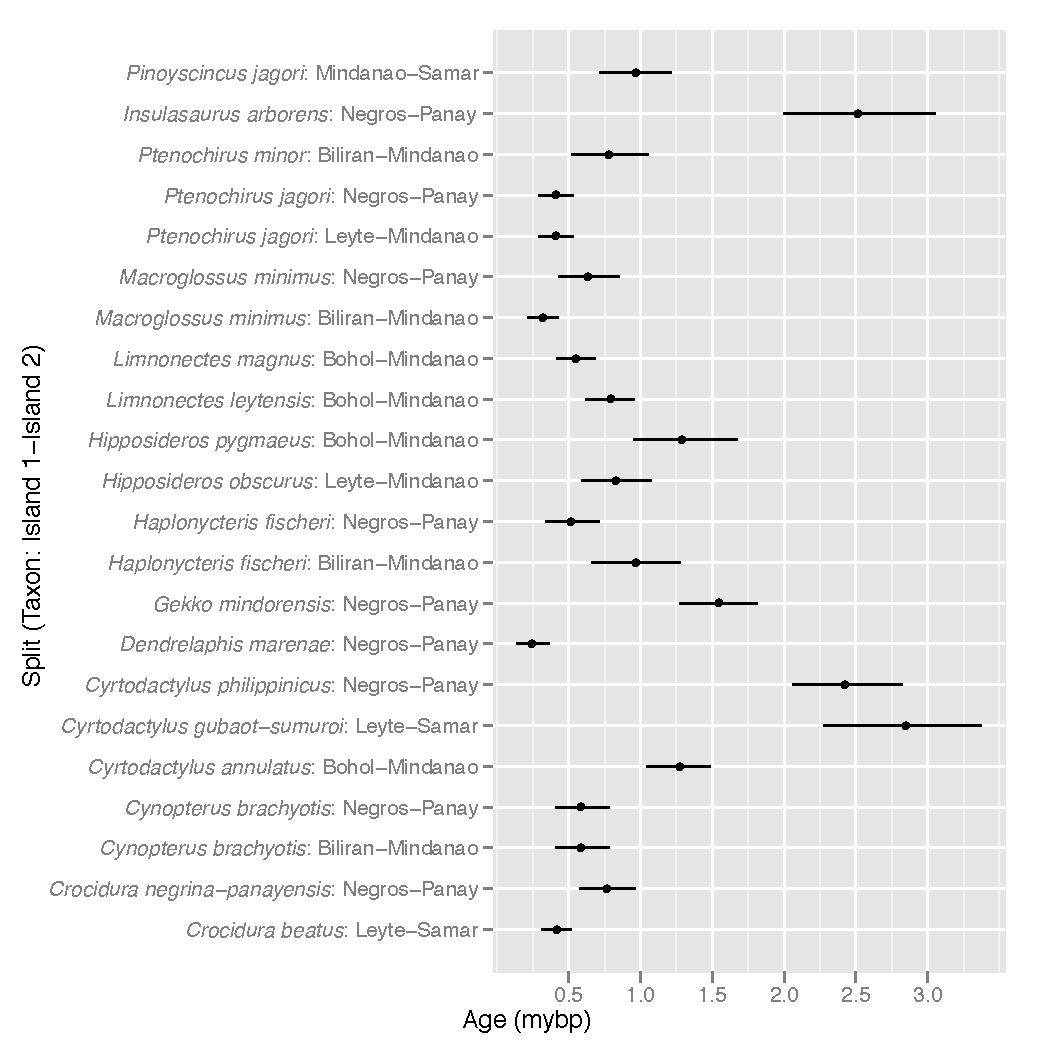
\includegraphics[height=8cm]{images/gene_splits.pdf}}
\end{frame}

\end{document}

